\documentclass{exam}
\usepackage{subfig}
\usepackage[utf8]{inputenc}
\usepackage{multirow}
\usepackage{url}
\usepackage{hyperref}
\usepackage{array,multirow,graphicx}
\usepackage{pgfplots}
\usepgfplotslibrary{patchplots}
\usepackage{tikz}
\usepackage{tikzscale}
\usepackage{mathtools}
\usepackage{bm}
\usepackage{amsmath,amssymb}
\newcommand{\xI}[1]{\mathbf{x}^{(#1)}}
\newcommand{\ls}{\ell}
\newcommand{\x}[0]{\mathbf{x}}
\newcommand{\variance}{\sigma^2}

\usepackage{wrapfig}
\newcommand{\lz}{\vspace{0.5cm}}
\newcommand{\thetab}{\bm{\weights}}
\newcommand{\zero}{\mathbf{0}}
\newcommand{\Xmat}{\mathbf{X}}
\newcommand{\Kmat}{\mathbf{K}}
\newcommand{\ydat}{\mathbf{y}}
\newcommand{\id}{\boldsymbol{I}}
\newcommand{\Amat}{\mathbf{A}}
\newcommand{\Xspace}{\mathcal{X}}                                           
\newcommand{\Yspace}{\mathcal{Y}}
\newcommand{\natnum}{\mathbb{N}}
\newcommand{\intnum}{\mathbb{Z}}

%-------------------------------------------------------------
\title{Collection of AutoML multiple Choice Questions}

\begin{document}
	\maketitle
	%-------------------------------------------------------------------
	\section{Big Picture}
	%Here, the questions begin
	All questions require a single choice answer.
	\begin{questions}
		
		\question AutoML can help you to ...
		\begin{choices}
			\choice replace the job of someone by a machine.
			\choice enables efficient interdisciplinary projects.
			\choice increase the time for finishing ML projects.
			\choice apply ML without any knowledge about the risks of ML.
		\end{choices}
		
		\question AutoML is a hard problem because ... (among other reasons).
		\begin{choices}
			\choice every function evaluation is super cheap
			\choice we only have to tune a single hyperparameter
			\choice we need the same ML pipeline for each dataset
			\choice the search space can quite complex and large
		\end{choices}
		
		\question The CASH problem stands for ...
		\begin{choices}
			\choice Combined Algorithm Solving and Hashing.
			\choice Combined Algorithm Selection and Hyperparameter Optimization.
			\choice Combined Automated Selection of Heuristics.
			\choice Combined Automated Selection of Hyperparameters.
		\end{choices}
		
		\question  To apply AutoML to deep learning, we ...
		\begin{choices}
			\choice want to ultimately optimize in the joint space of architectures and hyperparameters.
			\choice first optimize the architectures and afterwards the hyperparameters.
			\choice irst optimize the hyperparameters and afterwards the architecture.
		\end{choices}
		
		\question In dynamic algorithm configuration, we ...
		\begin{choices}
			\choice select a configuration specifically to each instance at hand.
			\choice predict which configuration an algorithm should use.
			\choice search for fixed dynamic schedule of configurations.
			\choice learn a policy that predicts a configuration for a given algorithm state.
		\end{choices}
		
		\question To mitigate the risks of AutoML, we ...
		\begin{choices}
			\choice will build systems that will avoid all of these risks automatically.
			\choice will blame ML and not AutoML.
			\choice teach others about potential risks of ML and AutoML.
			\choice will never publish our code as open-source.
		\end{choices}
		
		\pagebreak
		%-------------------------------------------------------------------------------
		\section{Evaluation}
		Kahoot quiz from the video consulting hour: \url{https://create.kahoot.it/share/automlss20-w2/9239e560-d2d6-4063-91d3-1be13047ae41}
		\question Training Machine Learning Models is ...
		\begin{choices}
			\choice trivially easy.
			\choice fundamentally an optimization problem. % Correct
			\choice always cheap.
		\end{choices}
		
		\question Performance estimation of a model = performance estimation of an algorithm
		\begin{choices}
			\choice True
			\choice False % Correct
		\end{choices}
		
		\question Reason for bad learning curves include ...
		\begin{choices}
			\choice underfitting % Correct
			\choice overfitting % Correct
			\choice optimal hyperparameter settings
			\choice high bias   % Correct
		\end{choices}
		
		\question Choose all that apply:
		\begin{choices}
			\choice underfitting $\mapsto$ high bias in model % Correct
			\choice underfitting $\mapsto$ high variance in model
			\choice overfitting $\mapsto$ high bias in model
			\choice overfitting $\mapsto$ high variance in model % Correct
		\end{choices}
		
		\question In a statistical hypothesis test with $\alpha = 0.05$ and $p < \alpha$ we
		\begin{choices}
			\choice Reject $H_0$ % Correct
			\choice Accept $H_0$
			\choice We cannot draw a conclusion.
		\end{choices}
		
		\question In a statistical hypothesis test with $\alpha = 0.05$ and $p > \alpha$ we
		\begin{choices}
			\choice Reject $H_0$
			\choice Accept $H_0$
			\choice We cannot draw a conclusion. % Correct
		\end{choices}
		
		\question Is it permissible to first look at your $p$ value before choosing your $\alpha$?
		\begin{choices}
			\choice Yes
			\choice No % Correct
		\end{choices}
		
		\question A parametric statistical hypothesis test makes distributional assumptions.
		\begin{choices}
			\choice True  % Correct
			\choice False
		\end{choices}
		
		\question Non-parametric test are (typically) more powerful compared to parametric tests (if applied correctly).
		\begin{choices}
			\choice True
			\choice False % Correct
		\end{choices}
		
		\question We need multi-test-correction because otherwise ...
		\begin{choices}
			\choice the probability of one test being wrong increases with the number of tests % Correct
			\choice the probability of one test being wrong decreases with the number of tests
			\choice it will increase the chance of rejecting $H_0$.
			\choice otherwise the number of required samples gets too large.
		\end{choices}
		
		\question An AutoML approach uses for its internal optimization
		\begin{choices}
			\choice the test set to estimate the generalization error.
			\choice the train set to avoid peaking at the test set.
			\choice the validation set to estimate the generalization error. % Correct
			\choice nested re-sampling to get a more reliable generalization estimate. % Correct
		\end{choices}
		
		\question For two algorithms X and Y we list their classification performance in the following table, with $0$ indicating a wrong classification and $1$ indicating correct classification.
		\begin{center}
			\begin{tabular}{cc|cc}
				& & \multicolumn{2}{c}{X} \\
				& & $0$ & $1$ \\
				\hline
				\multirow{2}{*}{Y} & $0$ & 30 & 90 \\
				& $1$ & 75 & 5 \\
			\end{tabular}
		\end{center}
		Use the McNemar Test where the \texttt{$H_0$: both models have the same performance} and \texttt{$H_1$: performances of the models are not equal}  with $\alpha = 0.05$\footnote{$\chi^2_1 = 3.841$}
		% Chi^2 = 1.188
		\begin{choices}
			\choice Reject $H_0$
			\choice Accept $H_0$
			\choice We cannot draw a conclusion. % Correct
		\end{choices}
		
		\question Instead consider now a different performance table with the rest being equal.
		\begin{center}
			\begin{tabular}{cc|cc}
				& & \multicolumn{2}{c}{X} \\
				& & $0$ & $1$ \\
				\hline
				\multirow{2}{*}{Y} & $0$ & 30 & 3 \\
				& $1$ & 17 & 5 \\
			\end{tabular}
		\end{center}
		% 17 + 3 <= 20 -> We shouldn't use McNemar
		\begin{choices}
			\choice Reject $H_0$
			\choice Accept $H_0$
			\choice We cannot draw a conclusion.
			\choice We shouldn't use McNemar % Correct
		\end{choices}
		
		\question The post-hoc Nemenyi test ...
		\begin{choices}
			\choice should be used before the Friedman test.
			\choice is used to determine if algorithms have the same ranks.
			\choice compares all pairs of algorithms to find best-performing algorithm after $H_0$ of the
			Friedman-test was rejected. % Correct
			\choice can not be used with more than 2 algorithms.
		\end{choices}
		
		\pagebreak
		%-------------------------------------------------------------------------------
		\section{Algorithm Selection}
		
		\question In algorithm selection we ...
		\begin{choices}
			\choice learn a mapping of algorithm to problem instance.
			\choice learn a mapping of problem instance to algorithm. % Correct
		\end{choices}
		
		\question Algorithm portfolios ...
		\begin{choices}
			\choice ideally contain very similar algorithms.
			\choice combine algorithms with complementary strengths. % Correct
			\choice should never contain more than $3$ algorithms.
			\choice minimize the risk of poor performance. % Correct
		\end{choices}
		
		\question With a \textit{good} algorithm selector we ...
		\begin{choices}
			\choice can only perform as good as the single best algorithm.
			\choice can only perform as good as the virtual best algorithm. % Correct
			\choice will likely have a performance better than the single best but worse than the virtual best algorithm. % Correct
		\end{choices}
		
		\question We should prefer parallel portfolios over selection ...
		\begin{choices}
			\choice when enough resources are available and the problem is easily evaluated in parallel. % Correct
			\choice when algorithms already require parallel resources.
			\choice as it is guaranteed to be faster than algorithm selection.
			\choice as compute resources have gotten very cheap.
		\end{choices}
		
		\question To train an algorithm selector we generally ...
		\begin{choices}
			\choice only need representative features of the problem instances.
			\choice require runtime data of the some algorithms on most of the problem instances.
			\choice have to evaluate all algorithms in the portfolio on all problem instances of a representative dataset. % Correct
			\choice only need enough data to determine the single best algorithm.
		\end{choices}
		
		\question Problem instance features ...
		\begin{choices}
			\choice related properties of datasets to algorithm performance. % Correct
			\choice generally do not require domain expertise.
			\choice can not be computed by running a representative algorithm for a short time / on a subset of the data.
			\choice are not important to learn an algorithm selector. Algorithm features are informative enough.
		\end{choices}
		
		\question Probing features usually lead to much better results than using just syntactic and information-theoretic features.
		\begin{choices}
			\choice True  % Correct
			\choice False
		\end{choices}
		
		\question Algorithm selection without problem features is impossible.
		\begin{choices}
			\choice True
			\choice False % Correct
		\end{choices}
		
		\question In practice ...
		\begin{choices}
			\choice all features are equally informative.
			\choice only very complex features are useful.
			\choice often only a small subset of the features are needed. % Correct
		\end{choices}
		
		\question Consider the following table containing the classification accuracies of $3$ different ML models.
		\begin{center}
			\begin{tabular}{cc|ccc}
				& & \multicolumn{3}{c}{Algorithm} \\
				& & SVM & CNN & kNN \\
				\hline
				\multirow{5}{*}{\rotatebox[origin=c]{90}{Dataset}} & $0$ & $0.59$ & $0.61$ & $0.55$\\
				& $1$ & $0.92$ & $0.93$ & $0.89$\\
				& $2$ & $0.32$ & $0.97$ & $0.75$\\
				& $3$ & $0.87$ & $0.80$ & $0.88$\\
				& $4$ & $0.95$ & $0.93$ & $0.65$\\
			\end{tabular}
		\end{center}
		Which statements are true?
		\begin{choices}
			\choice The single best algorithm is CNN.  % Correct
			\choice The single best algorithm is SVM.
			\choice The oracle would never select kNN.
			\choice The oracle would select every algorithm at least once. % Correct
		\end{choices}
		
		\question Consider now the corresponding feature table containing two binary features.
		\begin{center}
			\begin{tabular}{cc|cc}
				& & \multicolumn{2}{c}{Feature} \\
				& & F1 & F2 \\
				\hline
				\multirow{5}{*}{\rotatebox[origin=c]{90}{Dataset}} & $0$ & 0 & 0\\
				& $1$ & 0 & 1\\
				& $2$ & 0 & 0\\
				& $3$ & 1 & 1\\
				& $4$ & 0 & 1\\
			\end{tabular}
			Based on these features, is it possible to learn a perfect selector?
			\begin{choices}
				\choice True
				\choice False % Correct  % Should not be possible as in the 01 case either SVM and CNN are not easy to distinguish from each other.
			\end{choices}
		\end{center}
		
		\pagebreak
		%-------------------------------------------------------------------------------
		\section{HPO Basics}
		\question We determine the optimal hyperparameters ...
		\begin{choices}
			\choice with respect to the generalization performance. % Correct
			\choice with respect to the training performance.
			\choice based on incomplete runs.
		\end{choices}
		
		\question Model parameters ...
		\begin{choices}
			\choice are optimized during training. % Correct
			\choice are inputs to the training.
			\choice are equivalent to hyperparameters.
		\end{choices}
		
		\question Hyperparameters ....
		\begin{choices}
			\choice are outputs of the training.
			\choice often control the complexity of a model. % Correct
			\choice can influence model parameters. % Correct
			\choice can never change during training.
		\end{choices}
		
		\question Examples of model parameters are ...
		\begin{choices}
			\choice learning rates for neural network training.
			\choice the number of neighbors in $k$NN.
			\choice neural network weights. % Correct
			\choice centroids of $k$-means\footnote{\url{https://en.wikipedia.org/wiki/K-means\_clustering\#Algorithms}}. %Correct.
			\choice number of layers in a neural network.
			\choice support vectors of an SVM. % Correct
			\choice coefficients of a linear model. % Correct
			\choice the reward function used in reinforcement learning.
		\end{choices}
		
		\question (Hyperparameter) Tuning is the process of finding good model hyperparameters $\lambda$.
		\begin{choices}
			\choice True % Correct
			\choice False
		\end{choices}
		
		\question The components of a tuning problem are:  % Trick question. All of them are true
		\begin{choices}
			\choice The dataset.
			\choice The learner (possibly: several competing learners?) that is tuned.
			\choice The learner’s hyperparameters and their respective regions-of-interest over which we optimize.
			\choice The performance measure, as determined by the application.
			\choice A (resampling) procedure for estimating the predictive performance according to the
			performance measure.
		\end{choices}
		
		\question The performance measure of the tuning problem has to be  identical to the loss function that defines the risk minimization problem for the learner.
		\begin{choices}
			\choice True
			\choice False % Correct.
		\end{choices}
		
		\question Tuning
		\begin{choices}
			\choice is easy because people properly document their machine learning models and extensively document their behaviour on a plethora of application domains.
			\choice is hard because it is viewed as a black-box problem. % Correct
			\choice only involves very simple configuration spaces.
			\choice is hard because of the common stochasticity of machine learning models. % Correct
		\end{choices}
		
		\question Grid search can be disadvantageous compared to random search if
		some hyperparameters have little or no
		influence on the model.
		\begin{choices}
			\choice True
			\choice False
		\end{choices}
		
		\question With a tuning budget of $16$ samples and four parameters ...
		\begin{choices}
			\choice both grid and random search will evaluate $2$ unique values per parameter.
			\choice grid search will most likely evaluate more values per parameter than random search.
			\choice random search will most likely evaluate $16$ unique values per parameter and grid search $2$. % Correct. GS evaluates budget^(1/parameters) unique values.
			\choice both random search and grid search will evaluate $16$ unique values per parameter.
		\end{choices}
		
		\question Evolutionary Algorithms ...
		\begin{choices}
			\choice are conceptually simple, yet powerful enough to solve complex problems. % Correct
			\choice can not handle categorical parameters.
			\choice are perfectly suited for expensive problems like HPO.
			\choice have quite a few control parameters which often require tuning. % Correct
		\end{choices}
		
		\question Default heuristics ...
		\begin{choices}
			\choice are the same thing as static default hyperparameters.
			\choice determine parameter values based on some heuristic. % Correct
			\choice are very difficult to use.
		\end{choices}
		
		
		\clearpage
		%-------------------------------------------------------------------------------
		\section{GPs}
		\question The prior and posterior are called conjugate distributions if ...
		\begin{choices}
			\choice they are in different probability distributions families.
			\choice they are in the same probability distribution family. % Correct
		\end{choices}
		
		\question The Gaussian family is self-conjugate with respect to a Gaussian likelihood function.
		\begin{choices}
			\choice True % Correct
			\choice False
		\end{choices}
		
		\question Gaussian Processes are advantageous as ...
		\begin{choices}
			\choice only cheap to compute mathematical operations are required when fitting a GP.
			\choice they can handle partial observations (censored data) easily.
			\choice for every test input $x$ , we get a distribution over the prediction $y$. % Correct
			\choice the posterior can be updated online. % Correct
		\end{choices}
		
		\question Order the following images of a posterior with increasing number of observations.
		\begin{figure}[h!]
			\centering
			\subfloat{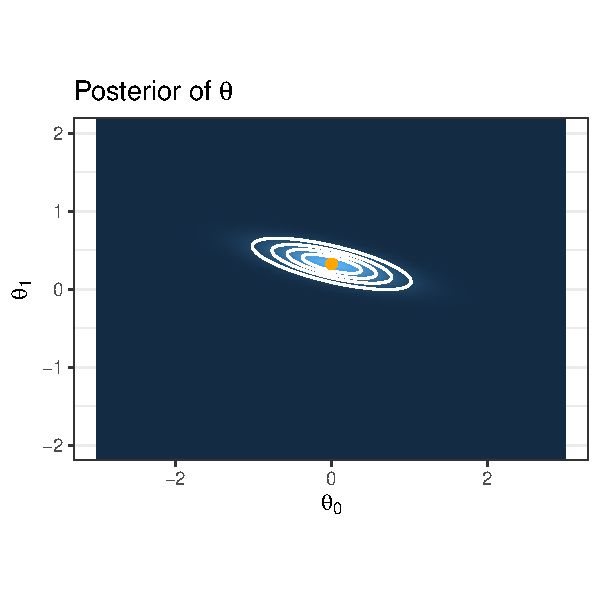
\includegraphics[width=.22\textwidth]{w05_gps/figure_man/bayes-lm/posterior-5-1.pdf}}
			\subfloat{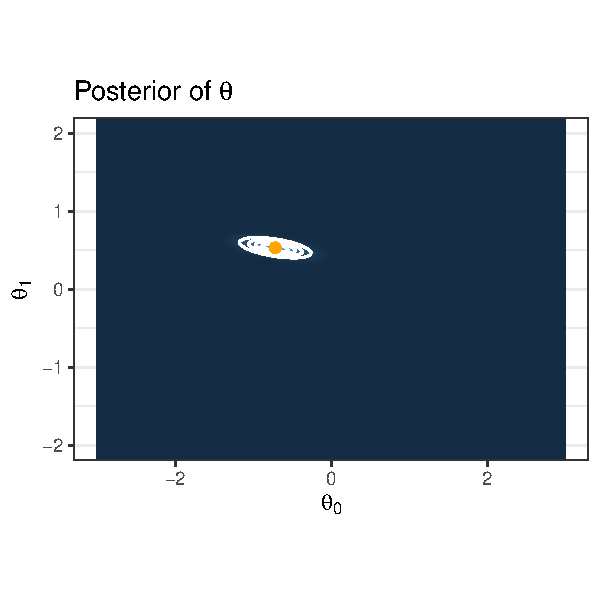
\includegraphics[width=.22\textwidth]{w05_gps/figure_man/bayes-lm/posterior-20-1.pdf}}
			\subfloat{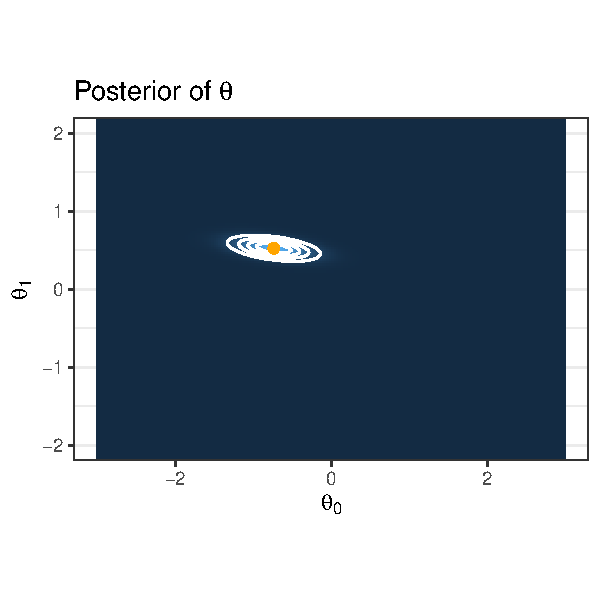
\includegraphics[width=.22\textwidth]{w05_gps/figure_man/bayes-lm/posterior-10-1.pdf}}
			\subfloat{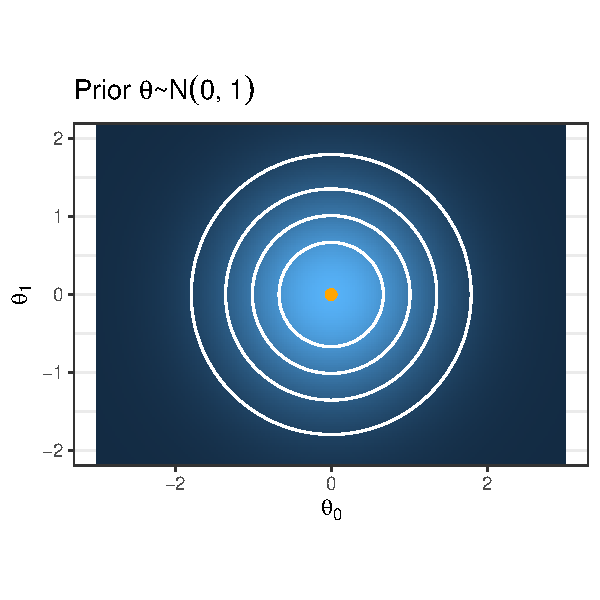
\includegraphics[width=.22\textwidth]{w05_gps/figure_man/bayes-lm/prior-1.pdf}}
		\end{figure}
		\begin{choices}
			\choice abcd
			\choice dcba
			\choice dabc
			\choice dacb % Correct
		\end{choices}
		
		\question Which kernel is most likely to have generated the following discrete samples\footnote{Note the figure title is no indicator to which answer is correct}:\\
		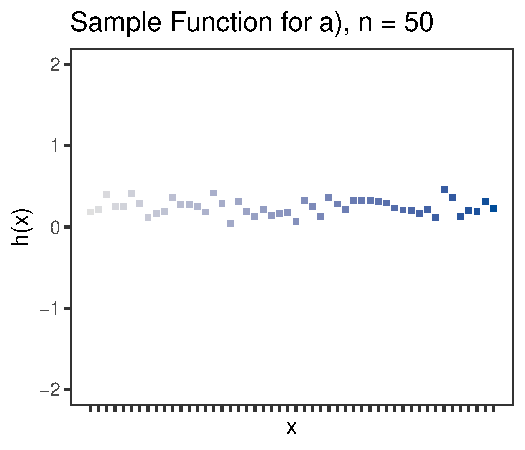
\includegraphics[width=.22\textwidth]{w05_gps/figure_man/discrete/example_extreme_50-1.pdf}
		\begin{choices}
			\choice $\bm{K} = \boldsymbol{I}$
			\choice $\bm{K} = \begin{footnotesize}\begin{pmatrix} 1 & 0.99 & ... & 0.99 \\
			0.99 & 1 & ... & 0.99 \\
			0.99 & 0.99 & \ddots & 0.99 \\
			0.99 & ... & 0.99 & 1 \end{pmatrix}\end{footnotesize}$ % Correct
			\choice \begin{footnotesize}$K_{ij} = k(\xI{i}, \xI{j}) = \exp\left(-\frac{1}{2}\left|\xI{i} - \xI{j}\right|^2\right)$\end{footnotesize}
		\end{choices}
		
		\question Which kernel is most likely to have generated the following discrete samples\footnote{Note the figure title is no indicator to which answer is correct}:\\
		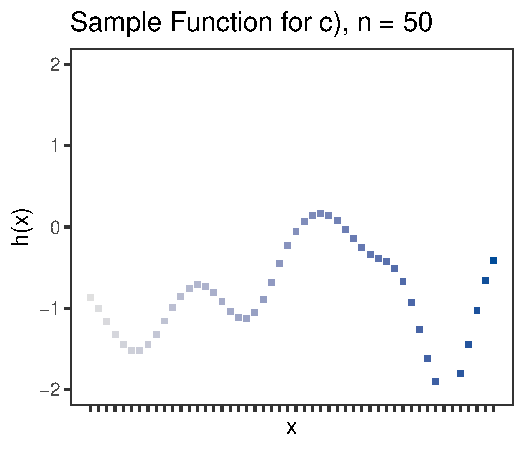
\includegraphics[width=.22\textwidth]{w05_gps/figure_man/discrete/example_extreme_50-3.pdf}
		\begin{choices}
			\choice $\bm{K} = \boldsymbol{I}$
			\choice $\bm{K} = \begin{footnotesize}\begin{pmatrix} 1 & 0.99 & ... & 0.99 \\
			0.99 & 1 & ... & 0.99 \\
			0.99 & 0.99 & \ddots & 0.99 \\
			0.99 & ... & 0.99 & 1 \end{pmatrix}\end{footnotesize}$
			\choice \begin{footnotesize}$K_{ij} = k(\xI{i}, \xI{j}) = \exp\left(-\frac{1}{2}\left|\xI{i} - \xI{j}\right|^2\right)$\end{footnotesize} % Correct
		\end{choices}
		
		\question Which kernel is most likely to have generated the following discrete samples\footnote{Note the figure title is no indicator to which answer is correct}:\\
		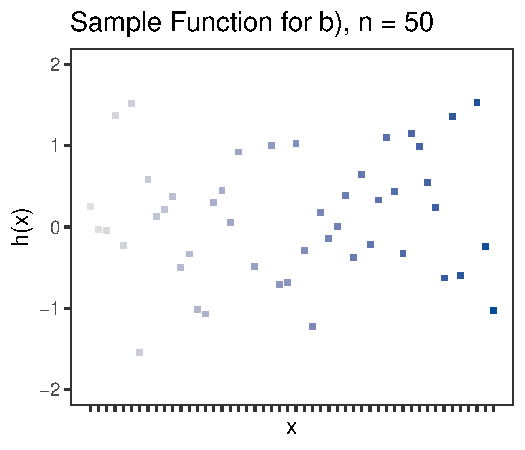
\includegraphics[width=.22\textwidth]{w05_gps/figure_man/discrete/example_extreme_50-2.pdf}
		\begin{choices}
			\choice $\bm{K} = \boldsymbol{I}$ % Correct
			\choice $\bm{K} = \begin{footnotesize}\begin{pmatrix} 1 & 0.99 & ... & 0.99 \\
			0.99 & 1 & ... & 0.99 \\
			0.99 & 0.99 & \ddots & 0.99 \\
			0.99 & ... & 0.99 & 1 \end{pmatrix}\end{footnotesize}$
			\choice \begin{footnotesize}$K_{ij} = k(\xI{i}, \xI{j}) = \exp\left(-\frac{1}{2}\left|\xI{i} - \xI{j}\right|^2\right)$\end{footnotesize}
		\end{choices}
		
		\question A GP is completely specified by its mean and covariance functions.
		\begin{choices}
			\choice True %Correct
			\choice False
		\end{choices}
		
		\question A Gaussian process is also an indexed family, where ...
		\begin{choices}
			\choice the input values $x\in\mathcal{X}$ are indexed by the random variables $f(x)$. 
			\choice the random variables $f(x)$ are indexed by the input values $x\in\mathcal{X}$. % Correct
		\end{choices}
		
		\question A kernel that only depends on $d = \x - \x'$ is ...
		\begin{choices}
			\choice stationary. % Correct
			\choice a dot product.
			\choice isotropic.
		\end{choices}
		
		\question A kernel that only depends on $r = ||\x - \x'||$ is ...
		\begin{choices}
			\choice stationary.  % Could also be accepted as isotropic implies stationary
			\choice a dot product.
			\choice isotropic. % Correct
		\end{choices}
		
		\question A kernel that only depends on $\x^{T}\x'$ is ...
		\begin{choices}
			\choice stationary.
			\choice a dot product. % Correct
			\choice isotropic.
		\end{choices}
		
		\question Consider the squared exponential kernel $\exp(- \frac{\|\x - \x'\|^2}{2\ls^2})$. Which of the following properties is true.
		\begin{choices}
			\choice The kernel is isotropic. %Correct
			\choice The kernel is a dot product.
			\choice The kernel is positiv definit. % Correct
		\end{choices}
		
		\question Consider the linear kernel $\variance_0 + \x^T\x'$. Which of the following properties is true.
		\begin{choices}
			\choice The kernel is isotropic.
			\choice The kernel is a dot product. % Correct
			\choice The kernel is positiv definit.
		\end{choices}
		
		\question the characteristic length-scale
		describes how far you need to move in input space for the function values to become
		uncorrelated.
		\begin{choices}
			\choice True % Correct
			\choice False
		\end{choices}
		
		\question The general rule of conditioning for Gaussians lets us
		\begin{choices}
			\choice talk about correlations only among training points.
			\choice talk about correlations among different test points. % Correct
			\choice sample functions from the posterior process. % Correct
			\choice makes online updates of GPs cheap.
		\end{choices}
		
		\question In the noise-free case the  ``prediction'' for a training point $\xI{i}$ is the exact function value $f(\xI{i})$.
		\begin{choices}
			\choice True % Correct
			\choice False
		\end{choices}
		
		\question In the noisy case a GP is still an interpolator. % Don't like the wording but used it to avoid "duplicate" to question above
		\begin{choices}
			\choice True
			\choice False % False
		\end{choices}
		
		\question When fitting a GP we ...
		\begin{choices}
			\choice only need to perform matrix computations. %Correct.
			\choice can learn the numerical hyperparameters of a selected kernel directly during GP training. % Correct
			\choice need at least $50D$ observations, where $D$ is the dimensionality of the target problem.
			\choice can \textbf{only} learn the length scale of a kernel directly.
		\end{choices}
		
		\question When training a GP ...
		\begin{choices}
			\choice we should always prefer a stationary kernel.
			\choice we can make use of a gradient based optimizer as the overhead of computing derivatives is small. % Correct
			\choice computing derivatives is the bottleneck.
			\choice inverting the kernel is the bottleneck. % Correct
		\end{choices}
		
		\question When assuming a non-zero mean GP prior ...
		\begin{choices}
			\choice both the predictive mean and variance change.
			\choice the mean takes the form $m(\Xmat_*) + \Kmat_*\Kmat_y^{-1}\left(\bm{y} - m(\Xmat)\right)$. % Corect.
			\choice the variance takes the form $\Kmat_{**} - \Kmat_*^T \Kmat ^{-1}\Kmat_*$. % Correct (if I haven't messed up the formula
			\choice both predictive mean and variance stay unchanged.
		\end{choices}
		
		
		\clearpage
		%-------------------------------------------------------------------------------
		\section{Bayesian Optimization for HPO}
		\question Categorical Hyperparameters ...
		\begin{choices}
			\choice depend on a parent hyperparemter.
			\choice are discrete and finite. % Correct
			\choice \textbf{always} have the same distance between values.
			\choice can not be optimized with GPs.
		\end{choices}
		
		\question In HPO we only have to deal with unstructured search spaces.
		\begin{choices}
			\choice True
			\choice False % Correct
		\end{choices}
		
		\question We can not parallelize bayesian optimization.
		\begin{choices}
			\choice True
			\choice False % Correct
		\end{choices}
		
		\question A good acquisition function ...
		\begin{choices}
			\choice emphasizes exploration.
			\choice emphasizes exploitation.
			\choice trades off exploration and exploitation. % Correct
		\end{choices}
		
		\question Expected Improvement vs Probability of Improvement.
		\begin{choices}
			\choice Both behave exactly the same, however PI is cheaper to compute.
			\choice EI emphasizes regions of large uncertainty, PI less. % Correct
		\end{choices}
		
		\question PI, EI, LCB/UCB and TS
		\begin{choices}
			\choice All given acquisition functions draw samples from the surrogate model to select the next query point.
			\choice All given acquisition functions use mean and uncertainty predictions to select the next query point.
			\choice Only TS draws samples from the surrogate model to select the next point. % Correct
			\choice PI, EI \& LCB/UCB use mean and uncertainty predictions to select the next query point. % Correct
		\end{choices}
		
		\question How would you set the exploration parameter for PI if you want to avoid too incremental improvements?
		\begin{choices}
			\choice Increase it over time. % Correct
			\choice Keep it constant.
			\choice Decrease it over time.
		\end{choices}
		
		\question KG is ...
		\begin{choices}
			\choice like EI after a 1-step look-ahead. % Correct
			\choice cheaper to compute than EI.
			\choice like PI after a 1-step look-ahead.
		\end{choices}
		
		\question ES ...
		\begin{choices}
			\choice reduces our uncertainty about the location of $\lambda^*$. % Correct
			\choice reduces our uncertainty about the performance of $\lambda^*$.
			\choice can only be computed using many samples.
		\end{choices}
		
		\question RF vs GP
		\begin{choices}
			\choice Gps should always be preferred over RFs.
			\choice RFs are preferable in high dimensions, for categorical spaces, or when function evaluations are quite fast. % Correct
			\choice Gps are preferable in low dimensional continuous spaces. % Correct
			\choice RFs should always be preferred over GPs.
		\end{choices}
		
		\question GPs can ...
		\begin{choices}
			\choice make use of low-effective dimensionalities through embeddings to... % Correct
			\choice never ...
			\choice use additive models on subsetsof dimensions to ... % Correct
		\end{choices}
		be applicable to problems with high dimensions.
		
		\question In practice evaluations always require the same amout of time.
		\begin{choices}
			\choice True
			\choice False
		\end{choices}
		
		\question When dealing with pending observations ...
		\begin{choices}
			\choice it is best to wait until all pending observations have arrived before continuing on.
			\choice ``hallucinated'' performance values can temporarily be used. % Correct
		\end{choices}
		
		\question What would happen if you treat a categorical hyperparameter as continuous(e.g.,{A,B,C}as{0,0.5,1}), in Bayesian optimization using a Gaussian Process?
		\begin{choices}
			\choice This is unproblematic as the GP would only make predictions at locations 0, 0.5 and 1.
			\choice This is problematic as the GP might suggest to evaluate at undefined locations. % Correct
			\choice This is problematic as this implies that there is a larger distance between A and C than A and B, whereas in reality the distance between the parameters is undefined. % Correct
			\choice This is unproblematic in this case as we preserve the order of the parameter values.
		\end{choices}
		
		\question With TPE ...
		\begin{choices}
			\choice we maintain a model of good configurations. % Correct
			\choice can not handle tree structured search-spaces.
			\choice maintain a model of bad configurations. % Correct
			\choice when optimizing $l(\lambda)/g(\lambda)$ is equivalent to optimizing standard expected improvement in BO. % Correct
		\end{choices}


\clearpage
%-------------------------------------------------------------------------------
\section{Speedup Techniques for Hyperparameter Optimization}
\question Black-box optimization ...
\begin{choices}
    \choice is the ideal view for HPO.
    \choice is too slow for expensive models. % Correct
    \choice can only handle up to $10$ parameters.
    \choice requires differentiable models.
\end{choices}

\question One method of going beyond BBO is ...
\begin{choices}
    \choice Sum of little black boxes     % Correct
    \choice Product of little black boxes  % A product would be too restrictive and could be dominated by only one of the little black boxes
\end{choices}

\question The best hyperparameter configuration ...
\begin{choices}
    \choice is highly dependent on the task and can not be transferred across tasks.
    \choice tends to quite stable across tasks. % Correct
    \choice can be transferred across tasks. % Correct
    \choice has to be determined only once and can be used on every new task.
\end{choices}

\question The goal of meta-learning is ...
\begin{choices}
    \choice to create descriptive features of datasets/tasks.
    \choice use only prior knowledge about a configuration to speed up solving of a new task.
    \choice is closely aligned with algorithm selection. %Correct
    \choice to use prior knowledge of dataset/task similarity and configuration performance to improve learning on new tasks. %Correct
\end{choices}

\question Select \textit{simple} meta-features used for meta-learning in ML
\begin{choices}
    \choice time related measures
    \choice standard deviation
    \choice number of features % correct
    \choice entropy
    \choice shape of a decision tree
    \choice number of classes % correct
\end{choices}

\question Model-Warmstarting ...
\begin{choices}
    \choice uses partially-trained models to determine which configuration to use.
    \choice uses predictive models of prior HPO runs to speed up HPO. %
\end{choices}

\question Joint models for BO ...
\begin{choices}
    \choice learn meta-features on all tasks jointly but have independent predictions per task. % Correct
    \choice learn the meta-features independently but have joint prediction (e.g. through voting).
\end{choices}

\question Learning a BBO algorithm ...
\begin{choices}
    \choice is impossible.
    \choice directly gives a mapping from data to hyperparameters. %Correct
    \choice always requires a differentiable black-box function.
\end{choices}

\question In the various meta-learning approaches, what will happen if all prior tasks are dissimilar to the target task?
\begin{choices}
    \choice A completely random hyperparameter configuration will be chosen.
    \choice The chosen meta-learning approach will get stuck in a dead-lock.
    \choice The chosen meta-learning approach will choose to apply a stable default configuration.
    \choice The configuration that worked best on a training task that most closely resembles the target task will be chosen. % Correct
\end{choices}

\question Multi-fidelity optimization ...
\begin{choices}
    \choice requires differentiable target algorithms.
    \choice only makes sense when dealing with large datasets.
    \choice exploits cheap approximations of expensife bb-functions. % correct
\end{choices}

\question It is important that the performance on low budgets correlates with performance on high budgets.
\begin{choices}
    \choice True % Correct
    \choice False
\end{choices}

\question How slow is Hyperband in the worst case?
\begin{choices}
    \choice As slow as Bayesian Optimization.
    \choice $10\times$ slower than random search.
    \choice as slow as random search. % Correct
    \choice as slow as grid search.
\end{choices}

\question BOHB ...
\begin{choices}
    \choice interleaves bayesian optimization and random search.
    \choice combines bayesian-optimization and hyperband. % Correct
    \choice builds a models for each fidelity to determine well performing configurations. % Correct
    \choice builds a model across all fidelities to determine well performing configurations.
\end{choices}

\question Partial learning curves ...
\begin{choices}
    \choice can be extrapolated to predict the final performance. % Correct
    \choice are hard to extrapolate as performance typically does drastically change during training. % Only true for RL
    \choice don't contain enogh information to be of use.
\end{choices}

\clearpage
%-------------------------------------------------------------------------------
\section{Multi-criteria Optimization}
\question The goal of multi-criteria optimization is ...
\begin{choices}
    \choice to optimize multiple target functions sequentially.
    \choice to optimize multiple target functions simultaneously. % Correct
    \choice to optimize multiple target functions independently in parallel.
    \choice to find the unique single best solution to a multi-class problem.
\end{choices}

\question Pareto front and Pareto set mean the same thing.
\begin{choices}
    \choice True
    \choice False % Correct
\end{choices}

\question A candidate $\lambda_1$ (Pareto-) dominates $\lambda_2$ if
\begin{choices}
    \choice $c_i(\lambda_1)\leq c_i(\lambda_2) \land c_j(\lambda_1) < c_j(\lambda_2)\quad\forall i \in \left\{1, 2, \ldots, m\right\} \exists j \in \left\{1, 2, \ldots, m\right\}$
    \choice $c_i(\lambda_1)\leq c_i(\lambda_2) \land c_j(\lambda_1) < c_j(\lambda_2)\quad\exists i \in \left\{1, 2, \ldots, m\right\} \forall j \in \left\{1, 2, \ldots, m\right\}$ % Correct
\end{choices}

\question Points on the Pareto front ...
\begin{choices}
    \choice are incomparable.
    \choice are dominated by all other datapoints.
    \choice dominate all other datapoints. % Correct
    \choice are equivalent. % COrrect
\end{choices}

\question Which of the following sections of the multi-objective cost-curve describe the pareto front?\\
(Hint: both objectives have to be minimized)
\begin{choices}
\begin{minipage}{\linewidth} 
\begin{wrapfigure}{r}{12.5cm}\vspace*{-.6cm}
    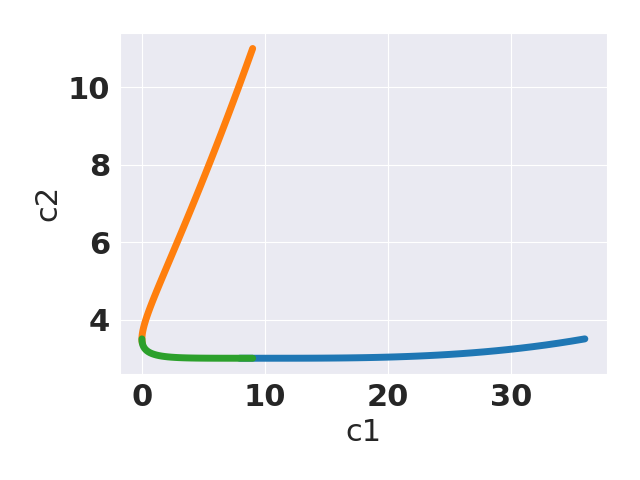
\includegraphics[width=.25\textwidth]{pareto_multi_choice.png}
\end{wrapfigure}
    \choice Blue
    \choice Green  % Correct
    \choice Orange
\end{minipage}
\end{choices}
\hfill\\

\question A-priori approaches ...
\begin{choices}
    \choice considers user preferences before the optimization process. % Correct
    \choice considers user preferences after the optimization process.
\end{choices}

\question The hypervolume ...
\begin{choices}
    \choice can only be used with EMOA ant not MO-BO.
    \choice can only be used with MO-BO ant not EMOA.
    \choice is useful to select the next query point. % Correct.
    \choice quickly becomes too expensive for ML applications to be used in practice.
\end{choices}

\question Drawbacks of scalarization (aggregation of all cost functions into one) include ...
\begin{choices}
    \choice requires expert knowledge to determine the best tradeoff. % Correct
    \choice difficult to implement.
    \choice simplification of multi-criteria optimization problem to single-objective
    \choice need to ensure that different trade-offs
between cost functions are explored. % Correct
\end{choices}		
	\end{questions}
\end{document}
